\documentclass{article}
\usepackage[margin=1in]{geometry}
\usepackage{amsmath,amsthm,amssymb}
\usepackage{bbm,enumerate,mathtools}
\usepackage{tikz,pgfplots}
\usepackage{chessboard}
\usepackage[hidelinks]{hyperref}
\usepackage{multicol} % Problem 35

\newenvironment{question}{\begin{trivlist}\item[\textbf{Question.}]}{\end{trivlist}}
\newenvironment{note}{\begin{trivlist}\item[\textbf{Note.}]}{\end{trivlist}}
\newenvironment{references}{\begin{trivlist}\item[\textbf{References.}]}{\end{trivlist}}
\newenvironment{related}{\begin{trivlist}\item[\textbf{Related.}]\end{trivlist}\begin{enumerate}}{\end{enumerate}}


\begin{document}
\rating{4}{2}
Consider ways to lay matchsticks (of unit length) on the $n \times m$ grid in
such a way that no end is ``orphaned''.
\begin{figure}[ht!]
  \centering
  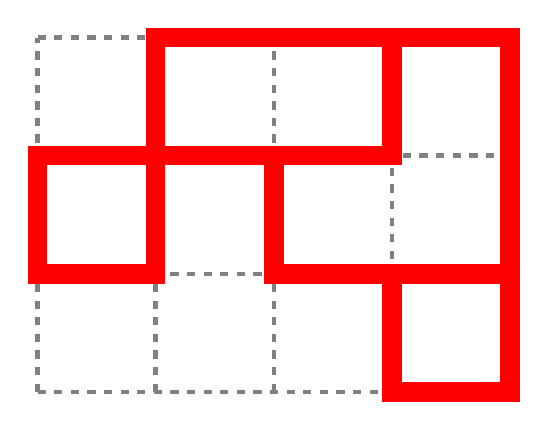
\begin{tikzpicture}[scale=1.5]
    \draw[ultra thick, gray, dashed] (0,0) grid (4,-3);
    \draw[line width=0.25cm, red] (2,-1)--(2,-2)--(3,-2);
    \draw[line width=0.25cm, red] (3,-0)--(3,-1)--(0,-1)--(0,-2)--(1,-2)--(1,-0)--(4,-0)--(4,-3)--(3,-3)--(3,-2)--(4,-2);
  \end{tikzpicture}\hspace{0.5cm}
  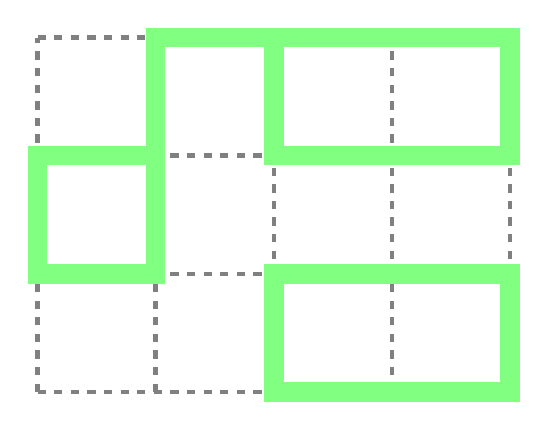
\begin{tikzpicture}[scale=1.5]
    \draw[ultra thick, gray, dashed] (0,0) grid (4,3);
    \draw[line width=0.25cm, green!50] (1,2)--(0,2)--(0,1)--(1,1)--(1,2)--(1,3)--(2,3)--(3,3)--(4,3)--(4,2)--(3,2)--(2,2)--(2,3);
    \draw[line width=0.25cm, green!50] (4,0)--(4,1)--(2,1)--(2,0)--cycle;
  \end{tikzpicture}
  \caption{
    Two examples of a valid configurations on a $5 \times 4$ grid; the second
    has an ``island'' in the lower right corner.
  }
\end{figure}
\begin{figure}[ht!]
  \centering
  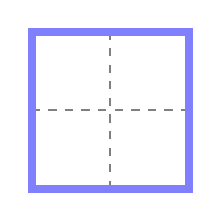
\begin{tikzpicture}
    \draw[thick, gray, dashed] (0,0) grid (2,2);
    \draw[line width=0.1cm, blue!50] (0,0) rectangle (2, 2);
  \end{tikzpicture}\hspace{0.5cm}
  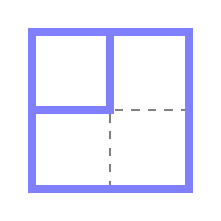
\begin{tikzpicture}
    \draw[thick, gray, dashed] (0,0) grid (2,2);
    \draw[line width=0.1cm, blue!50] (0,0) rectangle (2, 2);
    \draw[line width=0.1cm, blue!50] (0,1)--(1,1)--(1,2);
  \end{tikzpicture}\hspace{0.5cm}
  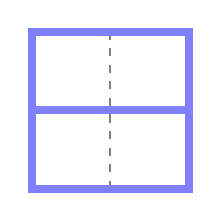
\begin{tikzpicture}
    \draw[thick, gray, dashed] (0,0) grid (2,2);
    \draw[line width=0.1cm, blue!50] (0,0) rectangle (2, 2);
    \draw[line width=0.1cm, blue!50] (0,1)--(2,1);
  \end{tikzpicture}\hspace{0.5cm}
  
\begin{tikzpicture}
    \draw[thick, gray, dashed] (0,0) grid (2,2);
    \draw[line width=0.1cm, blue!50] (0,0) rectangle (2, 2);
    \draw[line width=0.1cm, blue!50] (0,1)--(2,1);
    \draw[line width=0.1cm, blue!50] (1,0)--(1,2);
  \end{tikzpicture}\hspace{0.5cm}
  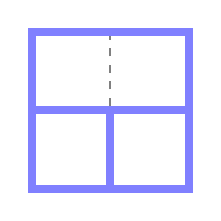
\begin{tikzpicture}
    \draw[thick, gray, dashed] (0,0) grid (2,2);
    \draw[line width=0.1cm, blue!50] (0,0) rectangle (2, 2);
    \draw[line width=0.1cm, blue!50] (0,1)--(2,1);
    \draw[line width=0.1cm, blue!50] (1,0)--(1,1);
  \end{tikzpicture}
  \caption{
    All(?) examples of valid configurations of $3 \times 3$ grids with
    border, up to dihedral action.
  }
\end{figure}
\begin{question}
  Let $a_\ell(n)$ be the number of configurations on the $\ell \times n$ grid.
  What is a general formula for $a_\ell(n)$?
\end{question}

\begin{related}
  \item What if the matchsticks are of length $k$?
  \item How does this generalize to a triangular/hexagonal lattice or to
    multiple dimensions?
  \item What is the number of these configurations with rotational symmetry?
    Horizontal/vertical symmetry?
  \item If such a configuration is chosen uniformly at random, what is the
    number of expected regions? (e.g. the first example has 4 interior
    regions.)
  \item What if no gridpoint can have degree 0? Degree 2? 3? 4?
  \item What if the entire border must be drawn?
  \item What if the the graph must be connected (i.e. cannot have an ``island''.)
  \item What if instead of horizontal/vertical lines, diagonals are allowed?
    All edges have integer slope?
    Edges don't intersect except at vertices?
  \item How many $k$-ominoes fit in a ``tube'' of height $m$? Snuggly?
\end{related}
\begin{references}
  \item The number of $2 \times n$ grids appears to be given by A093129.
  \item The number of $3 \times n$ grids is given by A301976.
\end{references}
\end{document}
